
% if you need a4paper uncomment this line
%\documentclass[a4paper, 12pt, conference]{ieeeconf}   

\documentclass[a4paper, 12pt, journal, onecolumn]{IEEEtran}
\usepackage{geometry}
\newgeometry{tmargin=3cm, bmargin=3cm, lmargin=3cm, rmargin=3cm}

\IEEEoverridecommandlockouts                       
%\overrideIEEEmargins
% See the \addtolength command later in the file to balance the column lengths
% on the last page of the document



% The following packages can be found on http:\\www.ctan.org
%\usepackage{graphics} % for pdf, bitmapped graphics files
%\usepackage{epsfig} % for postscript graphics files
%\usepackage{mathptmx} % assumes new font selection scheme installed
%\usepackage{times} % assumes new font selection scheme installed
%\usepackage{amsmath} % assumes amsmath package installed
%\usepackage{amssymb}  % assumes amsmath package installed

\title{\LARGE \bf
Report on Saluki: Finding Taint-style Vulnerabilities with Static Property Checking
}
\author{Jacek Janczura \\ \small{404975, Software Engineering of Embedded Systems, Technische Universitaet Berlin, {\tt janczura.jacek@gmail.com}}}%

\usepackage{graphicx} %package to manage images
\graphicspath{ {images/} }
%\usepackage{caption} % it throws the warning
\usepackage[style=base]{caption}
\usepackage{enumitem}

\usepackage[]{siunitx}
\usepackage{textcomp}

\usepackage{listings}
\usepackage{fancyhdr}
\fancyhf{}
\rhead{Jacek Janczura}
\lhead{Report on Saluki: Finding Taint-style Vulnerabilities }
\rfoot{Page \thepage}
\setlength{\headheight}{14pt}


\usepackage{xcolor}
\DeclareCaptionFont{white}{\color{white}}
\DeclareCaptionFormat{listing}{%
  \parbox{\textwidth}{\colorbox{gray}{\parbox{\textwidth}{#1#2#3}}\vskip-4pt}}
\captionsetup[lstlisting]{format=listing,labelfont=white,textfont=white}
\lstset{frame=lrb,xleftmargin=\fboxsep,xrightmargin=-\fboxsep}

\begin{document}

\maketitle
\thispagestyle{fancy}
\pagestyle{fancy}


%%%%%%%%%%%%%%%%%%%%%%%%%%%%%%%%%%%%%%%%%%%%%%%%%%%%%%%%%%%%%%%%%%%%%%%%%%%%%%%%
\begin{abstract}
\textbf{This report explains the architecture and Saluki's idea for checking taint-style (data dependent) security properties in a binary code. Saluki is a new tool which is capable of finding a large number of CWS\footnote{CWS- Common Weakness Enumeration - list of software weakness types \cite{a2}} vulnerabilities in real programs. Saluki uses a mixture of static and dynamic taint analysis to follow data dependent facts. Saluki is proved to be capable of finding vulnerabilities in COTS\footnote{ COTS - Commercial off-the-shelf -  products are packaged solutions which are then adapted to satisfy the needs of the purchasing organization \cite{a1}} including 0-days.}

\end{abstract}


%%%%%%%%%%%%%%%%%%%%%%%%%%%%%%%%%%%%%%%%%%%%%%%%%%%%%%%%%%%%%%%%%%%%%%%%%%%%%%%%
\section{INTRODUCTION}

Recently vendors continue to ship vulnerable programs. Unfortunately to protect their "know how" and intellectual property, source code is not shipped, which is a big issue. Modern compilers and run-time libraries have introduced significant complexities to a binary code, which negatively affect the capabilities of binary analysis tool kits to analyze binary code. \cite{binaries} To cope with analysing modern binary files, a data flow analysis is used for an accurate detection of a wide range of attacks on a shipped software, including those based on memory corruption, format-string bugs, command or SQL injection, cross-site scripting, and so on.(\cite{a7}, \cite{Pietraszek2006})

An example of data flow analysis used for finding such vulnerabilities is a taint analysis. The main goal of taint analysis is to identify data flows from attacker-controlled sources to security-sensitive sinks that do not undergo sanitization.\cite{a5} \cite{a6}
There are two types of taint analysis, dynamic and static. \cite{sdtaint} Dynamic requires run time support and can achieve low coverage, both of which can result in missed vulnerabilities. Static analysis, promises to reason about entire functions or whole programs at once by abstracting program state. As a result, static analysis tends to miss fewer problems, but can suffer high false positives if not done with care and is extremely time consuming. \cite{saluki} 

The solution for that problems is Saluki. This new tool, introduced by a research group from the Carnegie Mellon University, proposes the third approach - mixed taint analysis based on random execution. This type of data flow taint analysis is much faster than the conventional static approach and finds much more vulnerabilities than dynamic analysis.\cite{saluki} 

In this report after after introducing some basic concepts, we will focus on the Saluki's architecture, steps of its execution, some real life results and tests conducted using vulnerable binaries.
\pagebreak
%\section{Theoretical introduction}


\section{Control Flow Graph - CFG}

A CFG is defined to be a directed graph, consisting of vertices that represent basic blocks of the code and edges that represent control flow, $G = (V,E,V_e,V_x,T)$ , where: (\cite{CFG}, \cite{binaries})
\begin{itemize}
    \item $V = B ∪ \{v\perp\}$ is a set of nodes corresponding to all basic blocks $B$ and a special sink node $v\perp$ that has no instructions or outgoing edges;
    \item $E \subseteq V \times V$ is a set of control flow edges between nodes; 
    \item $V_e \subseteq V$ is a set of entry nodes;
    \item $V_x \subseteq V$ is a set of exit nodes;
    \item $ T : E \rightarrow \{intraprocedural, interprocedural\} $ assigns a label to an edge.

\end{itemize}
The basic blocks $B$ are defined in a conventional way. Each basic block $ b =< i_0, i_1, . . . , i_n > $ is a consecutive instruction sequence with $i_0$ being the only entry and in being the only exit. The sink node $v\perp$ is used to represent unknown control flows, mainly caused by indirect jumps and indirect calls.\cite{CFG2} An example of such graph is depicted in a Fig. \ref{fig:CFG}.

\begin{figure}[ht]
    \centering
    \captionsetup{justification=centering}
    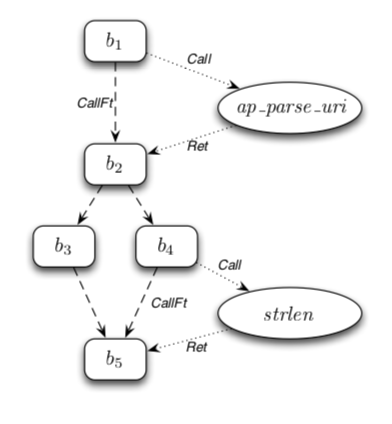
\includegraphics[width=0.6\textwidth]{CFG2.png}
    \caption{Sample Control Flow Graph.\\ Dashed arrows represent intraprocedural edges, while dotted arrows represent interprocedural edges. Functions are summarized as ellipses ($f$) \cite{CFG} }
    \label{fig:CFG}
\end{figure}

% \subsection{Approximation}

% Approximation stands for anything that is similar but not exactly equal to something else. In Fig. \ref{fig:approximation} a set of all possible states that can be achieved by the program during its execution is assigned with a letter A. To cover that set all the possible inputs needs to be supplied to the program, which will result in all of the possible states in the output. In other words, if all the possible inputs were supplied to the program, all the states from CFG will be reached. Unfortunately it is not possible to supply all of the potential inputs which is the reason for using the approximation. 

% \subsection{Under Approximation}

% Under approximation means that only the part of the possible states during the execution of the program are supplied. In that case it is not possible to cover all of the inputs but only the subset of them. The result of it is the subset of all the possible outputs. Under approximation in Fig. \ref{fig:approximation} is assigned with UA and is a subset of A. \cite{a4}

% \subsection{Over Approximation}

% Over approximation in case of achieving the CFG states, means that the set of the states in over approximation is bigger than the set of the all possible states that can be achieved by the program in CFB. Over approximation in Fig. \ref{fig:approximation} is assigned with OA and A is a subset of OA. \cite{a4}

% \begin{figure}[ht]
%     \centering
%     \captionsetup{justification=centering}
%     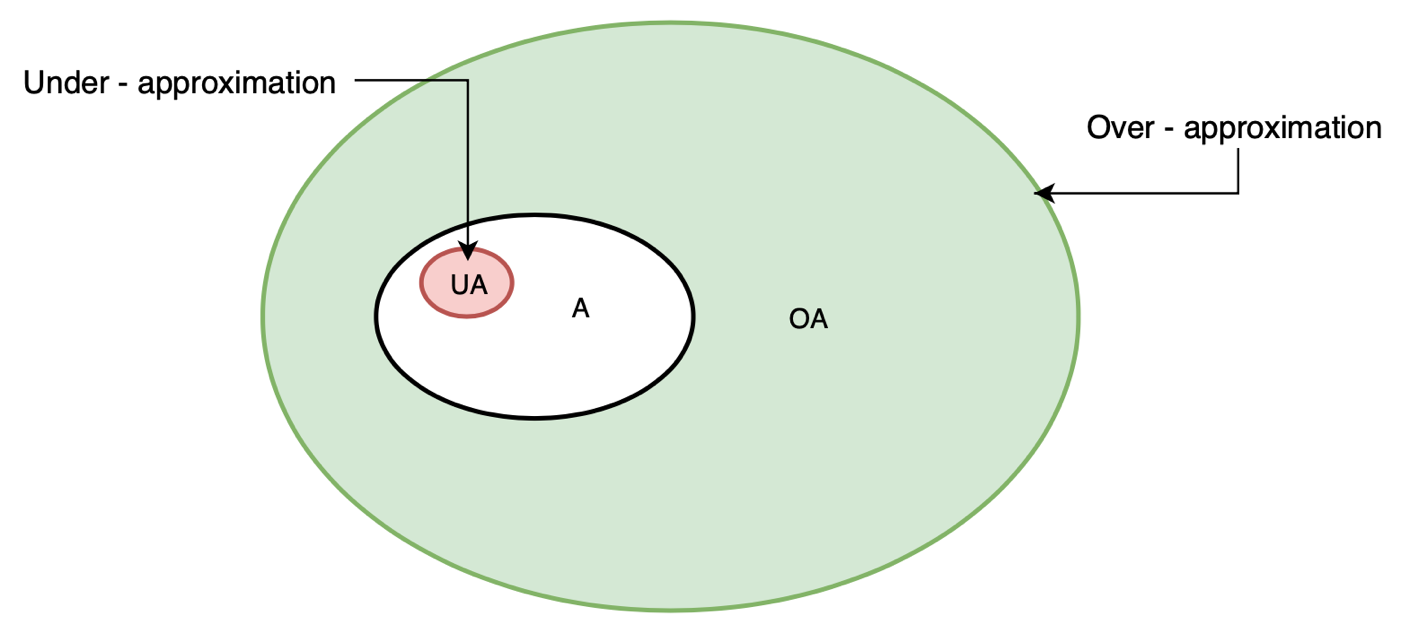
\includegraphics[width=0.8\textwidth]{approximation.png}
%     \caption{Visualisation of over and under approximation \cite{a3} }
%     \label{fig:approximation}
% \end{figure}

% \subsection{Mixed Approximation}

% Mixed approximation is a subset of the states that are reachable by the program and the states that are not possible to be reached in CFG.   

\section{Taint-style Vulnerabilities}


The term taint-style vulnerabilities has its roots in taint analysis, a technique for tracing  propagation of data through a program.\cite{a6} Taint analysis is based on the observation that in order for an attacker to change the execution of a program illegitimately, attacker must cause a value that is normally derived from a trusted source to instead be derived from his own input. We refer to data that originates or is derived arithmetically from an untrusted input as being tainted. \cite{taint2}

Taint analysis can be used for example to check if the data received to a socket by the function $receive()$ and saved in some buffer does not leak. It means that it is not sent away by the function $send()$.

In an example shown in a Fig. \ref{fig:taint}, functions and buffers that cannot be dependent one to another need to be specified. Any data saved by $receive(*buf_a)$ can not be sent away by $send(*buf_b)$. 
\\

Taint analysis is divided into three steps:\\
\begin{itemize}
\item \textbf{Seeding} - during seeding all the $receive()$ functions need to be find in the CFG. Than the memory cells, where the received data is saved, need to be tainted. Each tainted memory cell has its index number for tracing the leakage path and taint flag. Taint flag informs if that specific memory cell has been already tainted or not.\\
\item \textbf{Propagation} - taint propagation resembles spreading of a virus. In propagation step all the paths in CFG from $receive(*buf_a)$ to $send(*buf_b)$ are traversed and each used memory cell is tainted.\\
\item \textbf{Checking} - during checking each one of the memory cells in $buf_b$ is examined for the taint. Presence of the taint in $buf_b$ means that received data may be leaked away.\\
\end{itemize}

\begin{figure}[ht]
    \centering
    \captionsetup{justification=centering}
    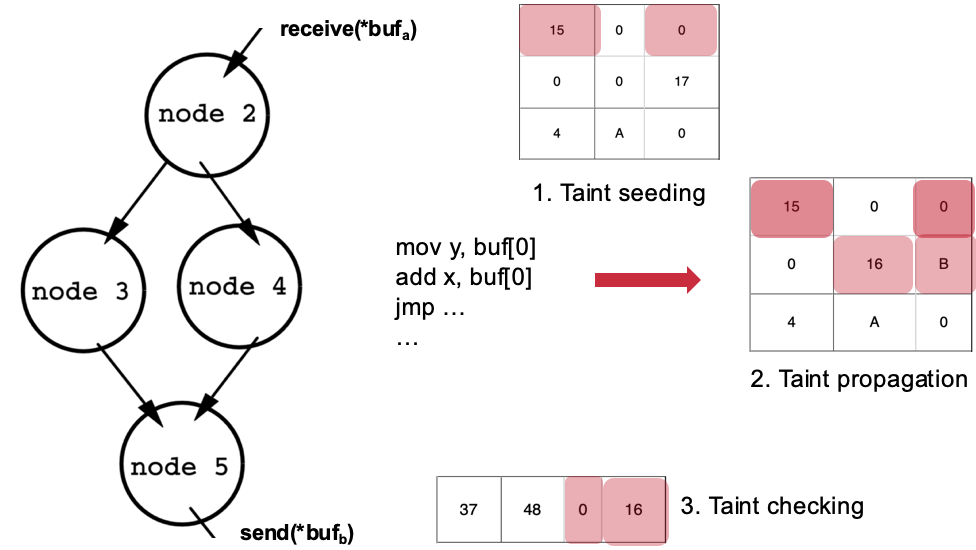
\includegraphics[width=0.9\textwidth]{Taint.png}
    \caption{Visualisation of taint analysis}
    \label{fig:taint}
\end{figure}

\subsection{Dynamic taint-style analysis}

In dynamic taint analysis, we first mark input data from un-trusted sources tainted, then monitor program execution to track how the tainted attribute propagates and to check when tainted data is used in dangerous ways. \cite{taint2}
Since dynamic analysis is done in a run time, by running the binary and following execution taint, for each different input whole program needs to be rerun from the beginning. In consequence to check all the possible states thus cover all the possible bugs the computational complexity of such approach will be extremely high and a scalability of it will be really poor. That is why in dynamic analysis only subset of the possible inputs is used to emulate working program. Therefore taint analysis is an example of an under approximation Fig.\ref{fig:approximation} and can not cover all of the possible vulnerabilities. \cite{a6}\cite{a7}

\begin{itemize}
\item Pros:	

\begin{itemize}
\item It is fast	
\item No false positive
\end{itemize}

\item Cons:

\begin{itemize}
\item Detects only bugs triggered by an executed path at the run time
\item Always starts at the entry point
\end{itemize}

\end{itemize}

\subsection{Static taint-style analysis}

Although static analysis examines all code paths, it has weakness of a high execution time. Due to it's content independency, static analysis  is possible to examine dead code that actually can not be executed in a run time. Consequently static taint-style analysis is an example of over approximation Fig.\ref{fig:approximation}.
Due to the large number of an external unreachable by the program in the run time states, in the static analysis we observe a large number of false positives. On the other hand all the states reachable by the program are the subset of the states reached by static analysis. It means that among many false positives, all of the possible bugs will be caught. \cite{a5}\cite{a6}

\begin{itemize}
\item Pros:	

\begin{itemize}
\item Detects all the bugs

\end{itemize}

\item Cons:

\begin{itemize}
\item Many false positives

\item Takes a long time
\end{itemize}

\end{itemize}

\begin{figure}[ht]
    \centering
    \captionsetup{justification=centering}
    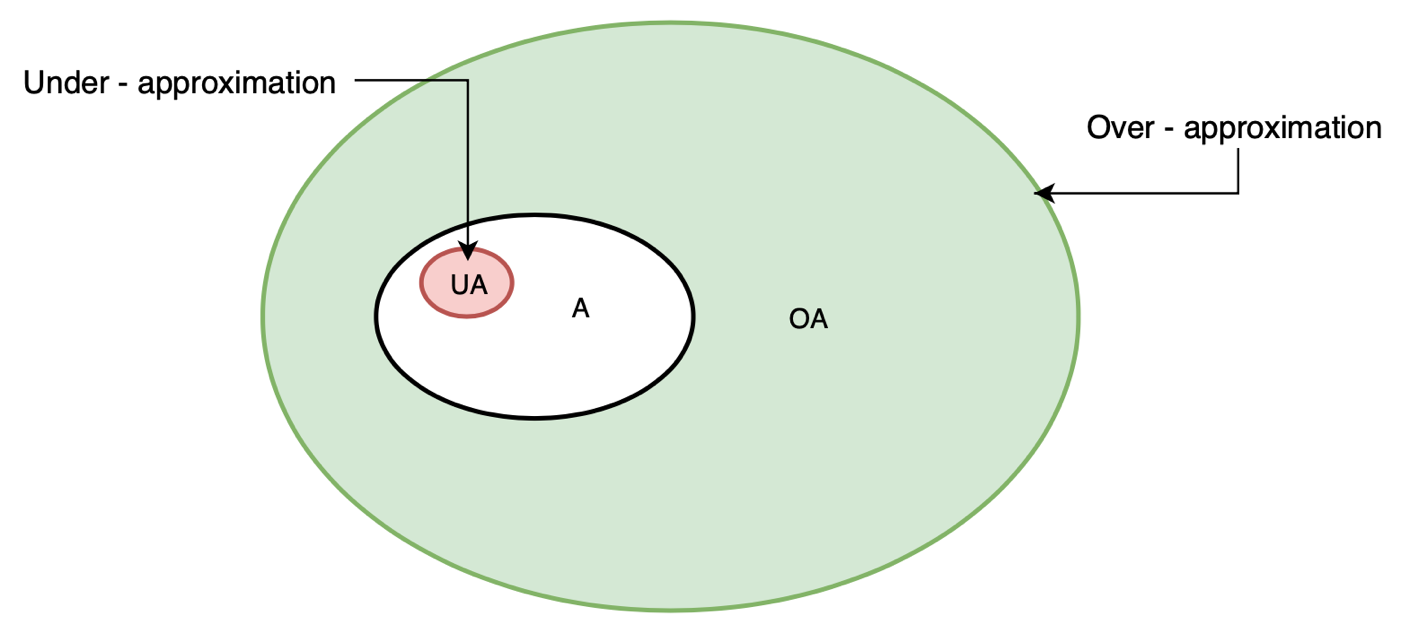
\includegraphics[width=0.8\textwidth]{approximation.png}
    \caption{Visualisation of over and under approximation. \\ A - a set of all the possible states of a binary, UA - an under approximation of A, OA - an over approximation of A \cite{a3} }
    \label{fig:approximation}
\end{figure}

\pagebreak

\section{Saluki Architecture}

Saluki creators came up with a new and novel approach. Instead of under approximating the states in a run time or statically slowly over approximating all the possible inputs and impossible states, in case of Saluki - random parts of code are executed. 

In a seeding part all instructions and policies that a user wants to check are being found in a control flow graph and tainted. Then in a propagation part, plugin called $\mu$flux executes random parts of the CFG supplying the random input and goes down the graph. 

Thanks to $\mu$flux and executing random parts of CFG, Saluki does not need to start every time from the beginning as it is in dynamic analysis. Additionally randomisation of an execution point, lets Saluki go as far as it is statistically possible in CFG, where in dynamic analysis going that deep entail extreme rise in the computational complexity. 

On the other hand randomisation of the input makes Saluki achieve a normally unreachable states like in over approximation. That is why the states approximation of Saluki is the mixed one.\cite{a4}
\\

Saluki's execution can be divided into five steps.
Its overall architecture is shown in a Fig. \ref{fig:saluki}.  \cite{saluki} :

\begin{enumerate}[label=\Alph*]
\item Load in the specification.
\item Parse the binary into an intermediate representation (IR\footnote{IR can be simplified for better understanding as creating a control flow graph of whole binary}) suitable for analysis. 
\item Run $\mu$flux\footnote{$\mu$flux works as a taint propagation} to collect data flow facts about executions from every specified source.
\item Run a solver over the policies, program, and collected facts. The solver determines whether the property holds or not.
\item Saluki outputs example paths where the property does not hold. The actual output is not a full path, but instead a condensed form of the tainted instructions and a flow ID.
\end{enumerate}

\begin{figure}[ht]
    \centering
    \captionsetup{justification=centering}
    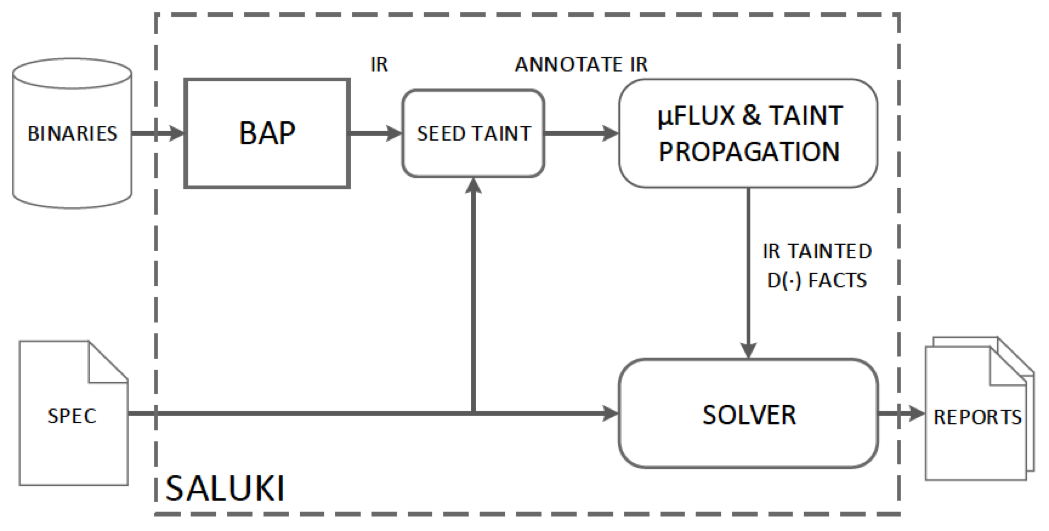
\includegraphics[width=0.85\textwidth]{saluki.png}
    \caption{Saluki Architecture \cite{saluki}}
    \label{fig:saluki}
\end{figure}

\textit{Specification: } The first step of running Saluki is loading the vulnerabilities specification. Saluki has already implemented a database - CWE\footnote{CWE - community-developed list of common software security weaknesses} with dozens of vulnerabilities. Additionally user can load customised, user-defined policies using the Saluki's language.\\

%\belowcaptionskip=-10pt

\begin{lstlisting}[label=saluki-code,caption=Command injection example]
    prop recv_to_system ::=
    recv(_,*buf,_,_), system(*cmd) |- never
    s.t. cmd/buf
\end{lstlisting}

In the Listing 1, there is shown a policy in Saluki language for finding a command injection. 

Command injection vulnerabilities arise when input flows from an input source to a sink function that executes code. 

In this case system should never use data from recv (data received from the socket). Otherwise we can assume that a command in a system shell was executed - system used data from the socket. 

The only limitation is that Saluki does not specifically reason about memory corruption vulnerabilities such as buffer overflows.
\bigskip

\textit{Binary processing:} The binary is loaded to the Saluki. Than Saluki runs a BAP\footnote{BAP - BinaryAnalysisPlatform - https://github.com/BinaryAnalysisPlatform/} (BinaryAnalysisPlatform) an open-source plugin-based binary analysis framework. Deriving a CFG from a binary is a difficult problem on its own right. The design of these algorithms is a challenge due to the presence of both indirect control flow that cannot be statically analyzed and data inter- mixed with code.\cite{CFG} To that purpose Saluki uses BAP recursive-traversal parser, that follows statically determinable control flow to discover as much code as possible, and makes use of backwards slicing and heuristic techniques to identify the targets of indirect jumps (e.g., jump tables) and functions that are only reached via indirect calls. (\cite{a8}, \cite{BAP})
\\

\textit{Taint Seeding:} Saluki analyzes the specification for variables used in constraints. Each constraint variable is linked to
a program location, which is then marked in the IR as a taint
seed. In our running example, cmd is a constraint variable used
in recv, causing Saluki to identify the proper memory location
corresponding to the cmd argument in all terms named recv.
As is customary, Saluki uses unique identifiers to identify each
taint seed.\cite{saluki}
\bigskip

\textit{$\mu$flux:} $\mu$flux is implemented as a custom interpreter that runs random parts of CFG and propagates the taint across the memory. $\mu$flux starts taint propagation from the instructions picked from specification and marked during the seeding. Than it executes parts of CFG randomly. $\mu$flux explores the paths regardless of the branch predicate and ignores context of data.
\medskip

$\mu$flux stops execution when:
\begin{itemize}
\item Pre-defined max. instructions number was excited
\item Saluki calls dynamically linked external function
\item Saluki hits a jump with an indirect target
\end{itemize}

\bigskip
\textit{The Saluki Solver:} In this step Saluki starts to follow the taint and tries to prove all properties specified in a policy. Saluki is constructive: it does not just show that there is a violation, but gives the specific path and data dependencies used to show the property can be violated.



\section{Results and tests}

Saluki research group tested Saluki on many binaries in order to check its performance. No only did they find two binaries where srand seed was time dependent and 6 new zero-days bugs in 5 COTS products, but they even discovered Heartbleed in OpenSSL. Unfortunately in the same library Saluki showed 4 false positive alerts.
In Lighthttp Saluki research team found command injection to system, buffer overflow due to wrong usage of strcpy. Apart from OpenSSL and Lighthttp they found 3 SQL injections in some COTOS products and many more.


This experiments shows that Saluki may be useful but the user needs to be aware that a false-positives may occur and that is why it is crucial to check every alert. 


\section{Conclusions}

Saluki is not sound nor complete. Its main advantage is that in comparison to other tools used to find vulnerabilities it is extremely fast. Unfortunately the authors of Saluki did not benchmark it against other tools which I think is a big drawback of the paper. 

Sadly Saluki is not further developed and after publication the paper \cite{saluki} there are no new commits in a Saluki's github repository. 

%%%%%%%%%%%%%%%%%%%%%%%%%%%%%%%%%%%%%%%%%%%%%%%%%%%%%%
\newpage

\bibliographystyle{unsrt}
\bibliography{sample}

\end{document}
